\documentclass[12pt]{article}
\usepackage[a4paper]{geometry}
\usepackage{fullpage}
\usepackage[T1]{fontenc}
\usepackage[utf8]{inputenc}
\usepackage{graphicx}
\usepackage{mathpazo}
\pagenumbering{gobble}
\usepackage{siunitx}
\sisetup{output-decimal-marker = {,}}
\usepackage{amsmath}
\usepackage{esdiff}
\usepackage{multicol}
\usepackage[spanish]{babel}

\begin{document}

\title{\textsc{Teoría de Circuitos III} :: Prueba BT1}

\date{4 de Octubre de  2018\\\small{Los resultados se publicarán el día 8 de octubre.\\La revisión del examen se realizará en horario de tutoría los días 9, 10 y 11 de octubre.}}

\maketitle

En el circuito de la figura el interruptor ha estado cerrado durante un tiempo elevado, y en $t = 0$ se abre. En estas condiciones se debe determinar:

\begin{enumerate}
\item (\textbf{1p.}) Tipo de transitorio presente en el circuito.

\item (\textbf{1p.}) Condiciones iniciales de las siguientes variables del circuito: $u_C(0^+)$, $i_L(0^+)$, $i_C(0^+)$, $u_{L1}(0^+)$.
\item (\textbf{1p.}) Valores en régimen permanente de las siguientes variables del circuito: $u_C(\infty)$, $i_L(\infty)$, $i_C(\infty)$, $u_{L1}(\infty)$.
\item (\textbf{6p.}) Expresiones de la corriente $i_L(t)$ y de la tensión $u_C(t)$ para  $t > 0$.

\item (\textbf{1p.}) Duración aproximada del transitorio. Si el tipo de transitorio produce oscilaciones, compare el período de la oscilación con la duración del transitorio.
\end{enumerate}

\begin{multicols}{3}

Datos:

$E_g = \SI{500}{\volt}$

$R_{1}= \SI{375}{\ohm}$%

$R_{2}=\SI{125}{\ohm}$%

$L_1 = \SI{40}{\milli\henry}$%

$L_2 = \SI{40}{\milli\henry}$%

$C = \SI{1}{\micro\farad}$%

\columnbreak

  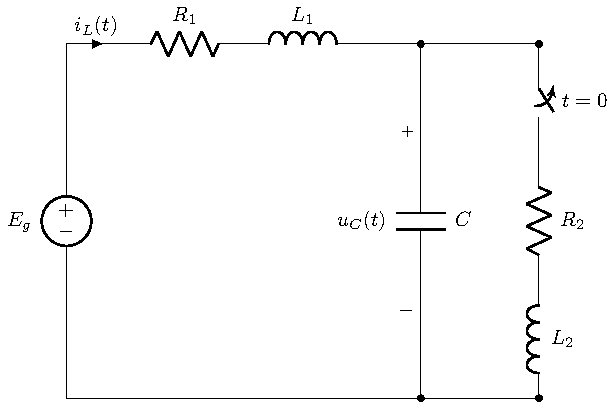
\includegraphics{figs/E1_RLC.pdf}

\end{multicols}

\clearpage

\subsection*{Solución}

\begin{enumerate}

\item Tipo de transitorio

La siguiente figura representa el circuito para $t > 0$.

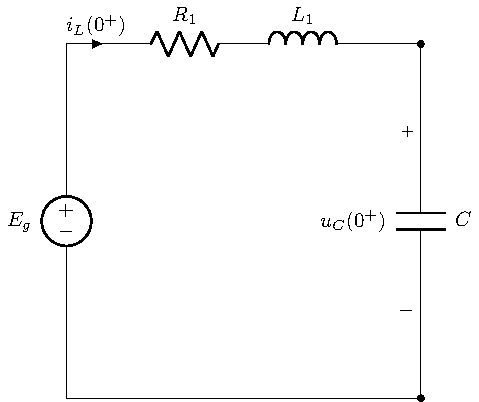
\includegraphics{figs/E1_RLC_0+.pdf}

Al apagar las fuentes en este circuito es evidente que se trata de un RLC serie. Por tanto podemos calcular:

\begin{align*}
  \alpha &= \frac{R}{2L} = \SI{4687.5}{\per\second}\\
  \omega_0 &= \frac{1}{\sqrt{LC}} = \SI{5000}{\radian\per\second}\\
\end{align*}

Dado que $\alpha < \omega_0$, el transitorio es subamortiguado.

\item Condiciones iniciales

  La siguiente figura representa el circuito para $t < 0$ en régimen permanente, con las variables particularizadas para $t = 0^-$.

  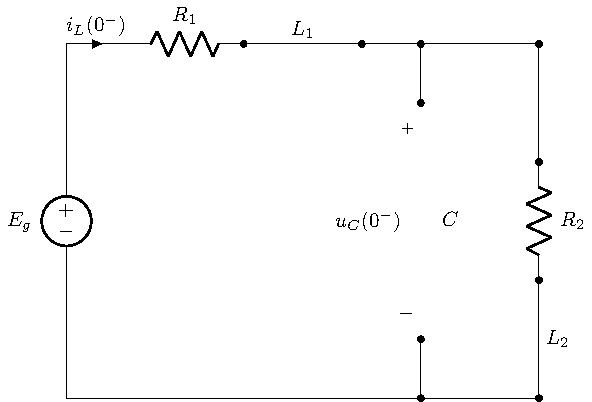
\includegraphics{figs/E1_RLC_0-.pdf}

  En este circuito, teniendo en cuenta las condiciones de continuidad, se puede deducir que:

  \begin{align*}
    i_L(0^+) = i_L(0^-) &= \SI{1}{\ampere}\\
    u_C(0^+) = u_C(0^-) &= \SI{125}{\volt}\\
  \end{align*}

  Además,
  \[
    E_g = u_R(0^+) + u_L(0^+) + u_C(0^+)
  \]

  Por tanto,

  \[
    u_L(0^+) = E_g - Ri_L(0^+) - u_C(0^+) = \SI{0}{\volt} 
  \]

  Finalmente, es evidente que $i_c(0^+) = i_L(0^+) = \SI{1}{\ampere}$.

\item Valores en régimen permanente.

  El circuito en régimen permanente está abierto debido al condensador. Por tanto,
  \begin{align*}
    u_c(\infty) & = \SI{500}{\volt}\\
    u_L(\infty) & = \SI{0}{\volt}\\
    i_c(\infty) & = \SI{0}{\ampere}\\
    i_L(\infty) & = \SI{0}{\ampere}
  \end{align*}

\item Expresiones de corriente y tensión

  La expresión genérica de la corriente es:

  \[
    i_L(t) = i(\infty) + e^{-\alpha t} \left(A_1 \sin(\omega_d t) + A_2 \cos(\omega_d t)\right)
  \]

  siendo $\omega_d = \sqrt{\omega_o^2 - \alpha^2} = \SI{1739.9}{\radian\per\second}$.
  
  Teniendo en cuenta las condiciones iniciales y el valor en régimen permanente obtenemos:

  \begin{align*}
    i_L(0^+) = 1 &= A_2\\
    \diff*{i_L}{t}{0^+} = \frac{1}{L}u_L(0^+) = 0 &= -\alpha A_2 + A_1 \omega_d
  \end{align*}

  La solución de este sistema es:

  \begin{align*}
    A_1 &= \frac{\alpha}{\omega_d} = 2.69\\
    A_2 &= 1\\
  \end{align*}
  
  Por tanto,
  \begin{align*}
        i_L(t) &= e^{-\alpha t} \left(\frac{\alpha}{\omega_d} \sin(\omega_d t) + \cos(\omega_d t)\right)\\
        i_L(t) &= e^{-4687.5 t} \left(2.69 \sin(1739.9t) + \cos(1739.9 t)\right)
  \end{align*}

  A partir de esta expresión podemos calcular la correspondiente a la tensión en el condensador teniendo en cuenta que:

  \[
    u_c(t) = E_g - R i(t) - L \diff{i}{t}
  \]
  Realizando la operación indicada obtenemos:

  \[
    u_C(t) = 500 - e^{-4687.5 t} \left(435.9 \sin(1739.9t) + 375 \cos(1739.9 t)\right)
  \]


  Este resultado se puede comprobar mediante las condiciones iniciales:

    \begin{align*}
    u_C(0^+) &= 125\\
    \diff*{u_c}{t}{0^+} &= \frac{1}{C}i_C(0^+) = 10^6\\
  \end{align*}

\item Duración del transitorio
  
  La duración del transitorio viene determinada por el factor que acompaña al tiempo en la exponencial, $\alpha = \SI{4687.5}{\per\second}$. Usando la regla de $5 \tau$, siendo $\tau = 1/\alpha = \SI{213.3}{\micro\second}$, podemos asumir que el transitorio se extinguirá al cabo de aproximadamente $\SI{1}{\milli\second}$.

  Al tratarse de un transitorio subamortiguado, presenta oscilaciones tal y como queda de manifiesto en las expresiones de la corriente y tensión. El período de estas oscilaciones se calcula a partir de la pulsación amortiguada:

  \[
    T_d = \frac{2\pi}{\omega_d} = \SI{3.61}{\milli\second} 
  \]
  Este valor, claramente superior a la duración del transitorio, implica que la oscilación no completará ni siquiera un ciclo (el transitorio se extinguirá alrededor de $T_d/4$).

\end{enumerate}

\end{document}

% Local Variables:
% ispell-local-dictionary: "castellano"
% End:

